\vspace{1 cm}
\begin{minipage}{\textwidth}
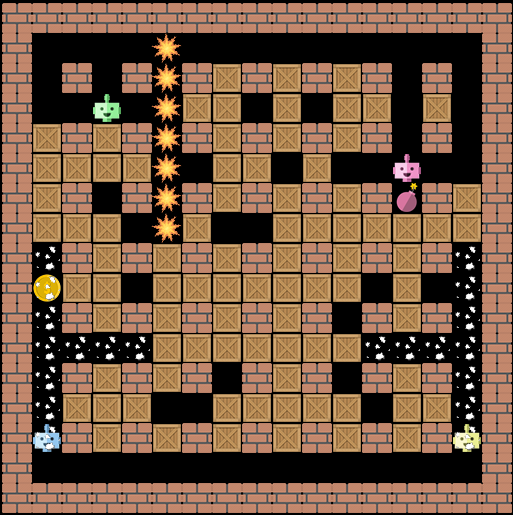
\includegraphics[scale=0.3]{./images/augmented_original.png}
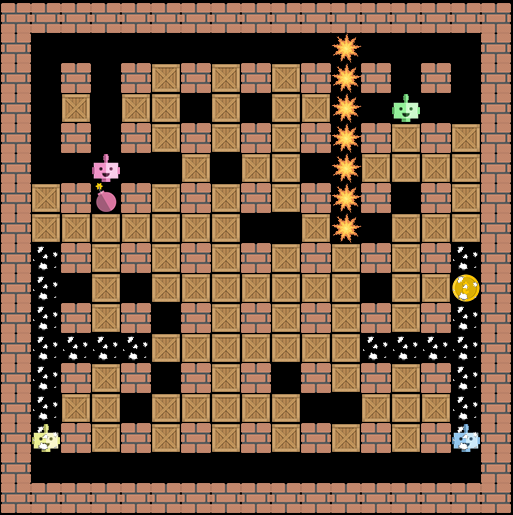
\includegraphics[scale=0.3]{./images/augmented_lr.png}
\end{minipage}
\begin{minipage}{\textwidth}
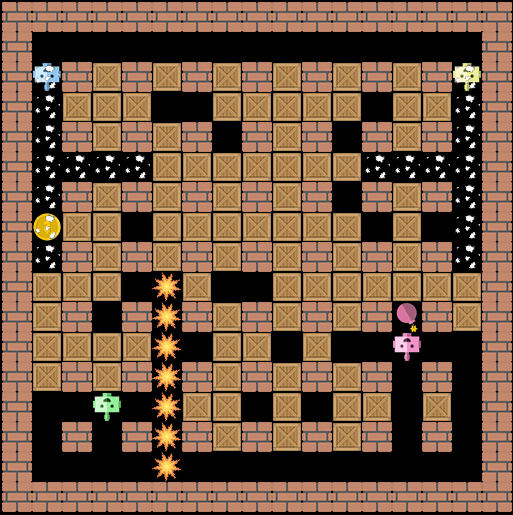
\includegraphics[scale=0.3]{./images/augmented_ud.png}
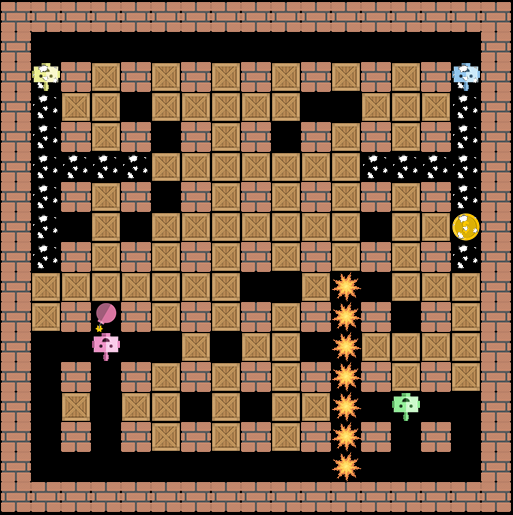
\includegraphics[scale=0.3]{./images/augmented_udlr.png}
\captionof{figure}{Data augmentation: \newline Upper left: original; Upper right: horizontal mirroring; \newline Lower left: vertical mirroring; Lower right: combined mirroring}
\label{fig:augmented}
\end{minipage}
\newline
\newline
\newline
\newline
As the inputs for our bomberchamp agent are symmetric, we wanted to use data augmentation to increase the number of samples for training and to make learning more symmetric.
From each original sample, three augmented samples were created. For augmentation, we had to mirror the environment and to change action choices accordingly. The augmented environment consisted of horizontal mirroring, vertical mirroring and a combination of both as seen in figure \ref{fig:augmented}.
For horizontal mirroring the agent choices left and right were exchanged, for vertical mirroring up and down and for the combination both were swapped. \newline
Data augmentation did not work as well as we expected, so it was not included in our final implementation.